\documentclass[a4paper,11pt,fleqn]{article}%fleqn pour aligner les equations à gauche
\usepackage{../../Styles/Exercice}


\newcommand{\chnum}{Chapitre 7}
\newcommand{\chtitle}{Equilibre acide-base}
\newcommand{\dtype}{Exercices}
  
\begin{document}
\maketitle

\begin{multicols}{2}
\section{pH d'une solution d'acide fort}
L'acide chlorhydrique est un acide fort dans l'eau. Une solution $S$ de concentration en soluté apporté $c$ = \SI{4,0E-2}{\mole \per \liter} est préparée.
\begin{enumerate}
	\item Rappeler la définition d'un acide fort
	\item Calculer le pH de la solution $S$
	\item Calculer le pH de la solution $S'$, obtenue en diluant par deux la solution $S$
\end{enumerate}

\section{pH d'une solution de base forte}
La potasse caustique (\ce{K+(aq)};\ce{HO-(aq)}) est une base forte dans l'eau. Une solution $S$ est préparée en dissolvant une masse $m$ = \SI{3,9}{\gram} de \ce{KOH(s)} dans un volume $V$ = \SI{100}{\milli \liter}.
\begin{enumerate}
	\item Calculer la masse molaire $M(\ce{KOH})$ à l'aide d'un tableau périodique
	\item Calculer la concentration $c$ en soluté apporté
	\item Écrire l'équation de la réaction de dissolution de l'hydroxyde de potassium \ce{KOH(s)} dans l'eau.
	\item Déterminer la concentration [\ce{HO-}]
	\item Calculer la concentration en ion oxonium dans la solution. En déduire le pH de la solution $S$
	\item La solution $S$ est diluée dix fois. Déterminer l pH de la solution $S'$ ainsi obtenue.
\end{enumerate}

\section{Constante d'acidité}
On prépare une solution d'hydrogénosulfate de sodium, (\ce{Na+(aq)};\ce{HSO4-(aq)}) de concentration $c$ = \SI{1,0E-2}{\mole \per \liter}.
\begin{enumerate}
	\item Écrire l'équation de dissolution de l'hydrogénosulfate de sodium dans l'eau
	\item Écrire l'équation de la réaction acide-base de l'ion hydrogénosulfate avec l'eau
	\item Exprimer la constante d'acidité du couple acide-base
	\item Le pH de cette solution est égal à \num{2,2}. En déduire les valeurs des concentrations de toutes les espèces chimiques présentes en solution et calculer la constante d'acidité
	\item En déduire son $pK_A$
\end{enumerate}

\section{Acide butyrique}
L'acide butyrique est aussi appelé acide butanoïque (\ce{C4H8O2}). C'est une molécule que l'on peut trouver dans le beurre rance ou le parmesan. Son odeur est forte et désagréable.
\begin{enumerate}
	\item Écrire la formule semi-développée de l'acide butanoïque.
	\item Écrire l'équation de la réaction de l'acide butanoïque avec l'eau
	\item Tracer le diagramme de prédominance du couple acide butanoïque/ion butanoate
	\item Le pH de l'estomac n'est pas constant. Lors d'une digestion idéale, il varie de 1,5 à 5. Préciser la ou les formes adoptées par l'espèce chimique lors de ces phases de digestion.
\end{enumerate}
\textbf{Donnée :} $pK_A$ du couple acide-base : $pK_A$ = 4,81

\section{Acide phosphorique}
L'acide phosphorique est un triacide de formule \ce{H3PO4} Les valeurs des trois $pK_A$ sont : 2,15 ; 7,20 et 12,3.
\begin{enumerate}
	\item Écrire les trois couples acide-base correspondant
	\item Représenter le diagramme de prédominance
	\item L'acide phosphorique est il un acide fort ?
	\item Comment qualifier l'ion \ce{H2PO4-(aq)} ?
\end{enumerate}

\section{Le cyanure}
L'ion cyanure est une base de formule \ce{CN-(aq)}. Les sels de cyanure ainsi que son acide conjugué sont très toxiques.
\begin{enumerate}
	\item Exprimer la constante d'acidité du couple
\end{enumerate}
On dispose de \SI{50}{\milli \liter} de solution à une concentration en soluté apporté $c$ = \SI{0,020}{\mole \per \liter}. Le pH de la solution est égal à 10,7.
\begin{enumerate}[resume]
	\item Conclure quant à la force de la base
\end{enumerate}

\section*{Exercice 7 : Aspirine}
L'aspirine est un acide faible dans l'eau, aussi appelé acide acétylsalicylique et noté ici \ce{AH(aq)}. On dissout un comprimé qui contient $m$ = \SI{500}{\milli \gram} d'aspirine dans un verre d'eau de volume $V$ = \SI{25}{\centi \liter}.
\begin{enumerate}
	\item Déterminer la concentration $c$ en soluté apporté
	\item Écrire l'équation de la réaction de l'acide acétylsalicylique avec l'eau et en déduire l'expression de la constante d'acidité.
	\item Le taux de dissociation d'une acide $\tau$ est défini comme le taux d'avancement de sa réaction avec l'eau : $\tau = \dfrac{x_f}{x_{max}}$.
	\begin{enumerate}
		\item Exprimer les concentrations $[\ce{AH}]_{\text{éq}}$, $[\ce{A-}]_{\text{éq}}$ et $[\ce{H3O+}]_{\text{éq}}$ en fonction de $c$ et $\tau$
		\item Établir que le taux de dissociation peut être calculé en résolvant l'équation du second degré : $c \cdot \tau^2 + K_A \cdot \tau - K_A = 0$
		\item Calculer $\tau$, puis le pH de la solution
		\item Déterminer la forme sous laquelle se trouve l'acide acétylsalicylique dans le verre
	\end{enumerate}
\end{enumerate}
\textbf{Données :}
\begin{itemize}
	\item Masse molaire de l'aspirine : $M$ = \SI{180,2}{\gram \per \mole}
	\item $pK_A$ du couple considéré : $pK_A$ = 3,5 
\end{itemize}

\section{Indicateur coloré}
Un flacon opaque d'un indicateur coloré est découvert, avec pour seules indications sa concentration en quantité de matière $c$ = \SI{2,90E-4}{\mole \per \liter} et son pH de 4,18. Le couple acide-base se cet indicateur coloré sera noté \ce{HInd}/\ce{Ind-}
\begin{enumerate}
	\item Déterminer la concentration en ion oxonium
	\item Déterminer le taux d'avancement de la réaction entre la forme \ce{HInd} et l'eau
	\item Établir que la constante d'acidité de l'indicateur coloré vaut $K_A$ = \num{1,9e-5}
	\item Identifier l'indicateur coloré retrouvé et la couleur de la solution à l'aide du tableau suivant.
\end{enumerate}
\begin{tabular}{|>{\centering}m{.17\linewidth}|>{\centering}m{.15\linewidth}|>{\centering}m{.15\linewidth}|>{\centering}m{.15\linewidth}|>{\centering\arraybackslash}m{.15\linewidth}|}
\hline Indicateur & Couleur acide & Zone de virage & Couleur basique & $pK_A$\\
\hline Héliantine & Rouge & 3,2 - 4,4 & Jaune orangé & 3,7\\
\hline Vert de bromocrésol & Jaune & 3,8 - 5,4 & Bleu & 4,7\\
\hline Bleu de bromocrésol & Jaune & 6,0 - 7,6 & Bleu & 7,0\\
\hline
\end{tabular}

\section{Arc-en-ciel végétal}
Certaines fleurs possèdent des pigments naturels dont la couleur dépend du pH. la couleur violette est due à une molécule amphotère que l'on note \ce{AH(aq)}.
\begin{enumerate}
	\item Écrire l'équation de la réaction de \ce{AH(aq)} en tant qu'acide avec l'eau
	\item Donner l'expression de la constante d'équilibre $K_{A2}$ de cette réaction, puis la calculer
	\item Le pH d'une solution contenant \ce{AH(aq)} est égal à 10. Exprimer littéralement le rapport $\dfrac{[\ce{A-}]_{\text{éq}}}{[\ce{AH}]_{\text{éq}}}$ et en déduire la couleur de la solution
	\item Écrire l'équation de la réaction de \ce{AH(aq)} en tant que base avec l'eau.
	\item Donner l'expression de la constante d'équilibre de la réaction en fonction de $K_{A1}$
	\item Réaliser le diagramme de prédominance des espèces \ce{AH2+(aq)}, \ce{AH(aq)} et \ce{A-(aq)}
	\item Déterminer le domaine de pH pour lequel la molécule est bleue
\end{enumerate}
\textbf{Données :}
\begin{itemize}
	\item $pK_A$ des espèces colorées : $pK_{A1}$ = 4,3 et $pK_{A2}$ = 7,0
	\item Couleur de \ce{AH2+(aq)} : rouge
	\item Couleur de \ce{AH(aq)} : violette
	\item Couleur de \ce{A-(aq)} : bleue
\end{itemize}

\section{Détermination d'un $pK_A$}
On souhaite déterminer expérimentalement le $pK_A$ d'un couple acide-base. Pour cela, on considère une solution placée dans le domaine de prédominance de l'acide. On suppose que la quantité de base est négligeable, et on note $n_0$ la quantité de matière de l'acide. À l'aide d'une burette, on ajoute progressivement une solution de soude (\ce{Na+(aq)} ; \ce{HO-(aq)}) et on mesure le pH de la solution au fur et à mesure. On notera $c_{soude}$ la concentration de la solution de soude.
\begin{enumerate}
	\item Écrire l'équation de la réaction ayant lieu
	\item À quel montage correspond cette expérience ?
	\item Comment repère-t-on le moment où les réactifs ont été introduits dans les proportions stœchiométriques ? On note $V_E$ le volume de soude versé correspondant.
	\item Écrire une relation vérifiée entre $V_E$, $c_{soude}$ et $n_0$
	\item La courbe obtenue pour le couple de l'acide éthanoïque \ce{C2H4O2(aq)}/\ce{C2H3O2-(aq)}. Déterminer le $pK_A$ de ce couple
\end{enumerate}
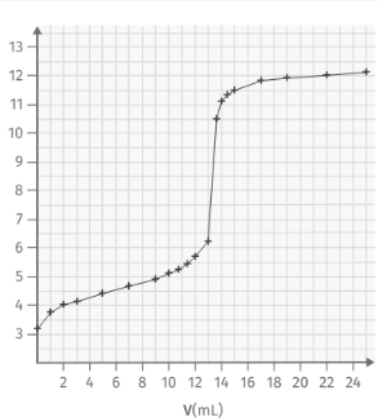
\includegraphics[width=\linewidth]{Ressources/TSPE_C8_Exercices_Fig1.png}
\end{multicols}
\end{document}